\subsection{Diagramma delle classi}
\label{subsec:diagramma_classi}

\begin{figure}[H]
    \centering
    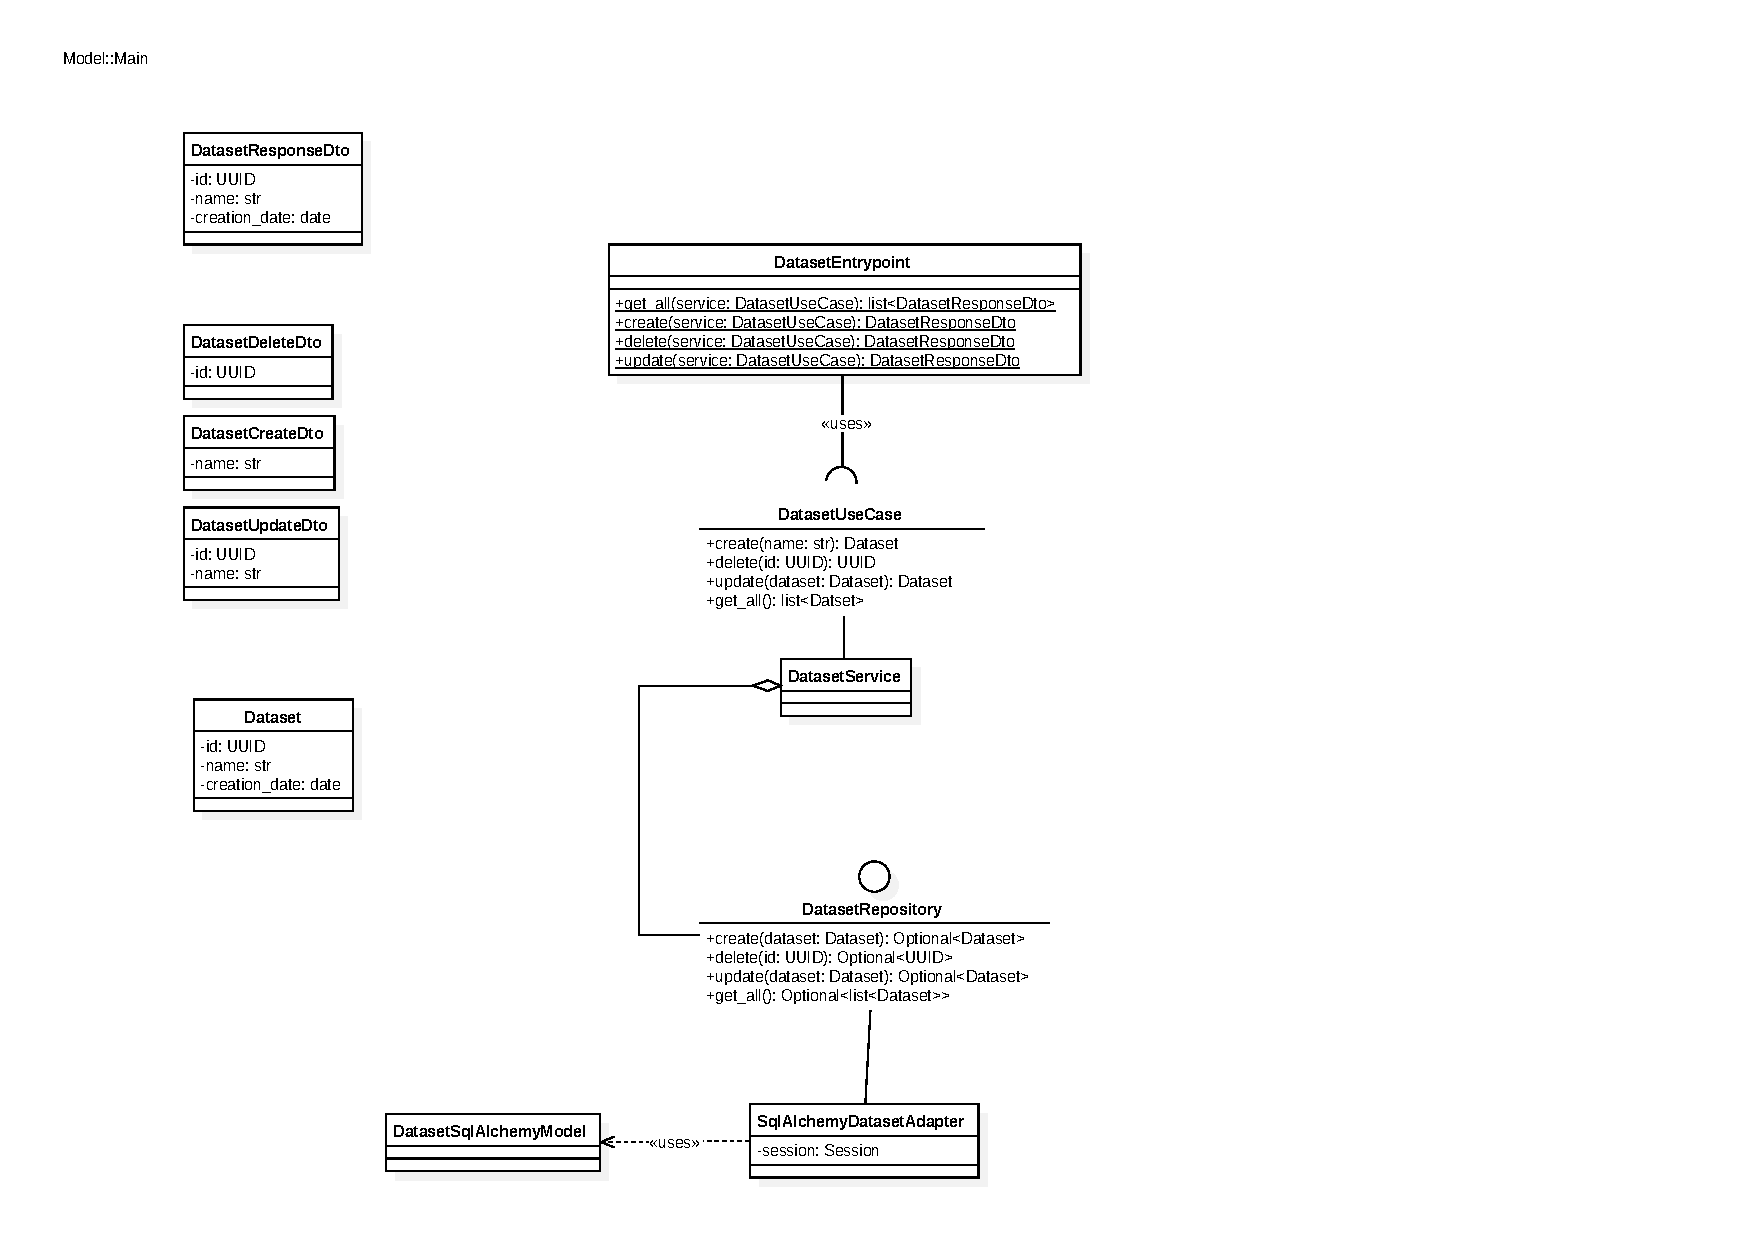
\includegraphics[width=1.8\textwidth]{Sezioni/ProgettazioneDettaglio/Immagini/Diagrammadataset.pdf}
    \caption{Diagramma delle classi relativo alla gestione dei Dataset}
    \label{fig:dataset_class_diagram}
\end{figure}


Il seguente diagramma rappresenta l'architettura software per la gestione dei \textit{Dataset}. Ogni componente ha un ruolo ben definito per garantire separazione delle responsabilità, scalabilità e manutenibilità.

\begin{itemize}
    \item \textbf{Dataset}: entità principale che rappresenta un dataset. Contiene i seguenti attributi:
    \begin{itemize}
        \item \texttt{id: UUID}, identificatore univoco del dataset.
        \item \texttt{name: str}, nome del dataset.
        \item \texttt{creation\_date: date}, data di creazione.
    \end{itemize}

    \item \textbf{DatasetRepository}: interfaccia che definisce le operazioni CRUD:
    \begin{itemize}
        \item \texttt{create(dataset: Dataset): Optional<Dataset>}
        \item \texttt{delete(id: UUID): Optional<UUID>}
        \item \texttt{update(dataset: Dataset): Optional<Dataset>}
        \item \texttt{get\_all(): Optional<list<Dataset>>}
    \end{itemize}

    \item \textbf{SqlAlchemyDatasetAdapter}: implementazione concreta del repository, basata su SQLAlchemy. Contiene:
    \begin{itemize}
        \item \texttt{session: Session}, sessione attiva con il database.
    \end{itemize}

    \item \textbf{DatasetSqlAlchemyModel}: modello ORM utilizzato da SQLAlchemy per mappare la classe \texttt{Dataset} sul database relazionale.

    \item \textbf{DatasetUseCase}: contiene la logica di business relativa ai dataset. I metodi esposti sono:
    \begin{itemize}
        \item \texttt{create(name: str): Dataset}
        \item \texttt{delete(id: UUID): UUID}
        \item \texttt{update(dataset: Dataset): Dataset}
        \item \texttt{get\_all(): list<Dataset>}
    \end{itemize}

    \item \textbf{DatasetService}: funge da intermediario e coordina il flusso delle richieste e delle risposte tra la DatasetRepository e la logica di business.

    \item \textbf{DTO (Data Transfer Object)}:
    \begin{itemize}
        \item \texttt{DatasetCreateDto} contiene \texttt{name: str}
        \item \texttt{DatasetDeleteDto} contiene \texttt{id: UUID}
        \item \texttt{DatasetUpdateDto} contiene \texttt{id: UUID}, \texttt{name: str}
        \item \texttt{DatasetResponseDto} contiene \texttt{id: UUID}, \texttt{name: str}, \texttt{creation\_date: date}
    \end{itemize}

    \item \textbf{DatasetEntrypoint}: rappresenta l'interfaccia esterna che permette di eseguire le operazioni sui dataset attraverso i casi d'uso. Metodi:
    \begin{itemize}
        \item \texttt{get\_all(service: DatasetUseCase): list<DatasetResponseDto>}
        \item \texttt{create(service: DatasetUseCase): DatasetResponseDto}
        \item \texttt{delete(service: DatasetUseCase): DatasetResponseDto}
        \item \texttt{update(service: DatasetUseCase): DatasetResponseDto}
    \end{itemize}
\end{itemize}

\subsubsection{Pattern architetturali utilizzati}
\label{subsubsec:pattern_architetturali}

Nel progetto sono stati adottati diversi pattern architetturali per garantire modularità, manutenibilità e facilità di test. Di seguito sono descritti i principali:

\begin{itemize}
    \item \textbf{Adapter Pattern} \\
    Il componente \texttt{SqlAlchemyDatasetAdapter} funge da adattatore tra l'interfaccia DatasetRepository e il sistema di persistenza. Come mostrato: da fare  
    \item \textbf{Entrypoint}
    Il componente \texttt{DatasetEntrypoint} funge da porta di ingresso e gestisce l'input esterno invocando i casi d'uso appropriati.

    \item \textbf{DTO (Data Transfer Object)} \\
    I DTO vengono utilizzati per trasferire dati tra i vari livelli dell'applicazione. Esempi sono:
    \begin{itemize}
        \item \texttt{DatasetCreateDto}, contenente i dati necessari alla creazione di un dataset;
        \item \texttt{DatasetUpdateDto}, per la modifica di un dataset;
        \item \texttt{DatasetResponseDto}, per il ritorno dei dati verso l'esterno.
    \end{itemize}

    \item \textbf{Dependency Injection} \\
    Il componente  \texttt{DatasetEntrypoint} utilizza il componente DatasetUseCase come parametro nei metodi, permettendo quindi di mantenere il core del dominio indipendente dalle implementazioni concrete delle classi.
\end{itemize}


\subsubsection{Descrizione delle funzioni e i metodi utilizzati}
